\documentclass{beamer}

\mode<presentation> {
\usetheme{Madrid}
}
\usepackage[utf8]{inputenc}
\usepackage[T1]{fontenc} 
\usepackage{graphicx}
\usepackage{xcolor}
\usepackage{listings}

\definecolor{mGreen}{rgb}{0,0.6,0}
\definecolor{mGray}{rgb}{0.5,0.5,0.5}
\definecolor{mPurple}{rgb}{0.58,0,0.82}
\definecolor{backgroundColour}{rgb}{0.95,0.95,0.92}

\lstdefinestyle{CStyle}{
    backgroundcolor=\color{backgroundColour},   
    commentstyle=\color{mGreen},
    keywordstyle=\color{magenta},
    numberstyle=\tiny\color{mGray},
    stringstyle=\color{mPurple},
    basicstyle=\footnotesize,
    breakatwhitespace=false,         
    breaklines=true,                 
    captionpos=b,                                         
    showspaces=false,                
    showstringspaces=false,
    showtabs=false,                  
    tabsize=2,
    language=C
}

\title[Linux Kernel Rootkit]{Linux Kernel Rootkit}

\author{Castets Nathan \& Huge Olivier}
\institute[UBX]{Université de Bordeaux}
\date{21 Février 2019}

\begin{document}

\begin{frame}
\titlepage
\end{frame}

\begin{frame}
\frametitle{Overview}
\tableofcontents
\end{frame}

\section{Notions et état de l'art des rootkits}
\subsection{Définitions}

\begin{frame}
\frametitle{Définitions}
\begin{block}{Rootkit}
Utilitaire qui permet d'effectuer différentes actions sur une machine. Le but principal est d'installer un accès privilégié à cette machine pour un pirate de façon persistante dans le temps.
\end{block}
\medskip
A la différence d'un malware classique, le rootkit se veut discret et dissimule au maximum ses actions à l'utilisateur et aux programmes de surveillance.
\end{frame}

\begin{frame}
\frametitle{Définitions}
Il existe 2 types de rootkit :
\begin{itemize}
\item 	Espace utilisateur\\
	Remplace des fonctions utilisées par un programme\\
	Injection de librarie dynamique via \textit{LD\_PRELOAD}
\item	Espace noyau\\
	Remplace des appels systèmes\\
	Module noyau qui écrase la table des appels systèmes
\end{itemize}
\end{frame}

\begin{frame}
\frametitle{Définitions}
\begin{block}{Table des appels systèmes}
Tableau contenant les adresses mémoires des fonctions associées aux appels systèmes. Ces appels systèmes permettent aux programmes de l'espace utilisateur de communiquer avec le noyau.
\end{block}
\medskip
Les appels systèmes sont indispensables pour les programmes de l'espace utilisateur pour utiliser des fonctions que seul le noyau peut exécuter.

On appelle aussi la table des appels systèmes la \textit{sys\_call\_table}.
\end{frame}

\begin{frame}
\frametitle{Définitions}
\begin{block}{KASLR}
La KASLR (Kernel Address Space Layout Randomization) est une sécurité du noyau qui charge aléatoirement les données dans la mémoire.
\end{block}

Cela implique qu'à chaque démarrage du système une structure de donnée n'est généralement pas à la même adresse.

C'est la sécurité principale qui empêche les rootkits de s'installer dans le système.
\end{frame}

\subsection{Pré Linux Kernel 4.17}

\begin{frame}[fragile]
\frametitle{Pré Linux Kernel 4.17}
/fs/open.c :
\begin{lstlisting}[style=CStyle]
/* *** */

EXPORT_SYMBOL(sys_close);

/* *** */
\end{lstlisting}
\medskip
La fonction associée à l'appel système \textit{sys\_close} est accessible par n'importe quel programme présent dans le noyau.

Cet export est présent car le module \textit{mount} a besoin de \textit{sys\_close}.

\medskip
Un brute-force de la mémoire noyau à la recherche des occurences de l'adresse de \textit{sys\_close} nous donne la \textit{sys\_call\_table}.
\end{frame}

\subsection{Post Linux Kernel 4.17}

\begin{frame}
\frametitle{Post Linux Kernel 4.17}
\begin{itemize}
\item 	Suppression de la majorité des appels systèmes dans le code noyau\\
	L'export de la fonction \textit{sys\_close} n'existe plus\\
\item 	Rajout de fonction avec un comportement similaire \textit{ksys\_xyzxyz()}\\
	Le but étant de dissocier au maximum les appels venants de l'espace utilisateur et noyau
\end{itemize}
Cela implique :
\begin{itemize}
\item 	Qu'il n'est plus possible de brute-force la \textit{sys\_call\_table} à l'aide de l'adresse d'un appel système
\item 	Qu'il n'est plus possible d'altérer le comportement de programme présent dans le noyau
\end{itemize}
\end{frame}

\section{Notre Rootkit}
\subsection{Déterminer l'adresse de la table des appels systèmes}

\begin{frame}
\frametitle{Déterminer l'adresse de la table des appels systèmes}
L'idée est de s'intéresser au fonctionnement des appels systèmes et plus précisément au code exécuté en préambule pour préparer l'appel système.

\medskip
Retracer ce code dans la mémoire noyau jusqu'à retrouver un offset vers la \textit{sys\_call\_table}.

\medskip
Nous nous concentrerons sur les version 4.17 à 4.20 du noyau Linux dans la suite de cette présentation.
\end{frame}

\begin{frame}[fragile]
\frametitle{Déterminer l'adresse de la table des appels systèmes}
Dès qu'un appel système est levé, le processeur doit exécuter du code pour préparer cet appel système. L'adresse de ce code se trouve dans le registre \textit{MSR\_LSTAR}. Voyons à l'initialisation ce que contient ce registre.

\medskip
/arch/x86/kernel/cpu/common.c (4.17 - 4.19) :
\begin{lstlisting}[style=CStyle]
if (static_cpu_has(X86_FEATURE_PTI))
	wrmsrl(MSR_LSTAR, SYSCALL64_entry_trampoline);
else
	wrmsrl(MSR_LSTAR, (unsigned long)entry_SYSCALL_64);
\end{lstlisting}

\medskip
/arch/x86/kernel/cpu/common.c (4.20) :
\begin{lstlisting}[style=CStyle]
wrmsrl(MSR_LSTAR, (unsigned long)entry_SYSCALL_64);
\end{lstlisting}
\end{frame}

\begin{frame}[fragile]
\frametitle{Déterminer l'adresse de la table des appels systèmes}
/arch/x86/entry/entry\_64.S (4.17 - 4.20) :
\begin{lstlisting}[style=CStyle]
ENTRY(entry_SYSCALL_64)
	/* *** */
	pushq	%rax

	PUSH_AND_CLEAR_REGS rax=$-ENOSYS
	TRACE_IRQS_OFF
	movq	%rax, %rdi
	movq	%rsp, %rsi
	call	do_syscall_64
	TRACE_IRQS_IRETQ
	movq	RCX(%rsp), %rcx
	movq	RIP(%rsp), %r11
	cmpq	%rcx, %r11
	jne	swapgs_restore_regs_and_return_to_usermode
\end{lstlisting}
\end{frame}
\begin{frame}[fragile]
\frametitle{Déterminer l'adresse de la table des appels systèmes}
/arch/x86/entry/common.c (4.17 - 4.20) :
\begin{lstlisting}[style=CStyle]
__visible void do_syscall_64(unsigned long nr, struct pt_regs *regs)
{
	/* *** */
	nr &= __SYSCALL_MASK;
	if (likely(nr < NR_syscalls)) {
		nr = array_index_nospec(nr, NR_syscalls);
		regs->ax = sys_call_table[nr](regs);
	}
	/* *** */
}
\end{lstlisting}
\end{frame}
\begin{frame}[fragile]
\frametitle{Déterminer l'adresse de la table des appels systèmes}
/arch/x86/entry/common.c (4.17 - 4.20) :
\begin{lstlisting}[style=CStyle]
static __always_inline void do_syscall_32_irqs_on(struct pt_regs *regs)
{
	/* *** */
	if (likely(nr < IA32_NR_syscalls)) {
		nr = array_index_nospec(nr, IA32_NR_syscalls);
	regs->ax = ia32_sys_call_table[nr](regs);
	/* *** */
}
\end{lstlisting}
\end{frame}
\begin{frame}
\frametitle{Déterminer l'adresse de la table des appels systèmes}
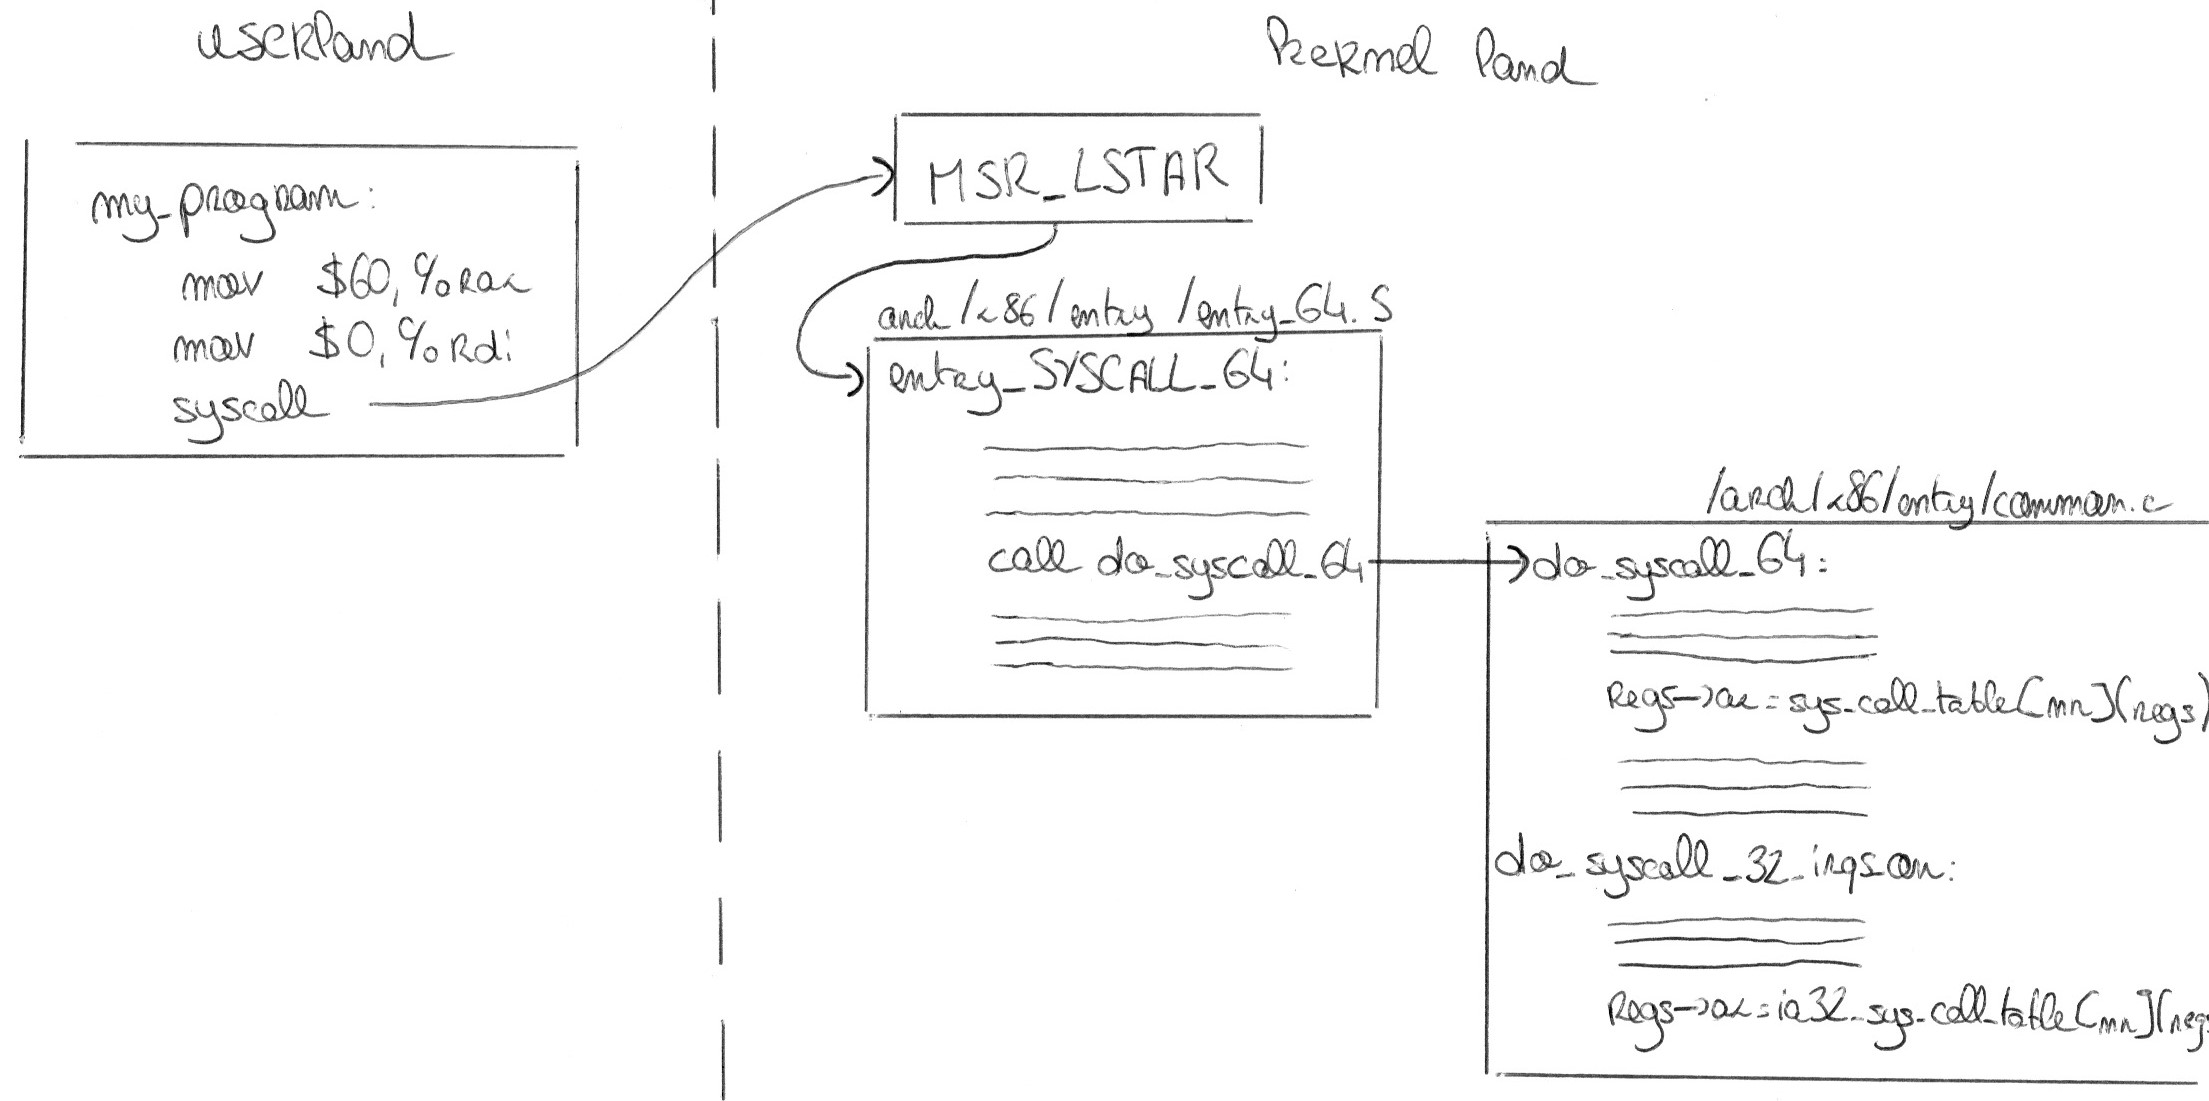
\includegraphics[scale=0.43]{figure}
\end{frame}
\subsection{Patterns pour retrouver l'offset de \textit{sys\_call\_table}}
\begin{frame}[fragile]
\frametitle{Patterns pour retrouver l'offset de \textit{sys\_call\_table}}
Tout d'abord il nous faut l'adresse de la fonction \textit{entry\_SYSCALL\_64} :
\begin{itemize}
\item 	En version 4.20 il nous suffit de lire le registre \textit{MSR\_LSTAR}
\item 	Dans les versions 4.17 - 4.19, on pourrait aussi lire le registre \textit{MSR\_LSTAR} et suivre le code exécuté jusqu'à atteindre \textit{entry\_SYSCALL\_64}
\end{itemize}
\begin{block}{Astuce}
La fonction \textit{native\_load\_gs\_index} qui se trouve juste en dessous de \textit{entry\_SYSCALL\_64} dans le code est exportée via un \textit{EXPORT\_SYMBOL}.
\end{block}
\end{frame}
\begin{frame}[fragile]
\frametitle{Patterns pour retrouver l'offset de \textit{sys\_call\_table}}
Dans \textit{entry\_SYSCALL\_64} on cherche l'appel à \textit{do\_syscall\_64} :
\begin{lstlisting}[style=CStyle]
e8 ?? ?? ?? ??       callq [offset]
\end{lstlisting}
\medskip
Il est précédé par les instructions suivantes :
\begin{lstlisting}[style=CStyle]
4.17 - 4.20
41 57                 push %r15  
45 31 ff              xor %r15d, %r15d  
48 89 c7              mov %rax, %rdi  
48 89 e6              mov %rsp, %rsi  
\end{lstlisting}
\end{frame}
\begin{frame}[fragile]
\frametitle{Patterns pour retrouver l'offset de \textit{sys\_call\_table}}
Dans \textit{do\_syscall\_64} on cherche l'appel à \textit{sys\_call\_table} :
\begin{lstlisting}[style=CStyle]
48 8b 04 fd ?? ?? ?? ?? mov [offset](, %rdi, 8), %rax
\end{lstlisting}
\medskip
Il est précédé par les instructions suivantes :
\begin{lstlisting}[style=CStyle]
4.17  
48 81 ff 4d 01 00 00  cmp $0x14d, %rdi  
48 19 c0              sbb %rax, %rax  
48 21 c7              and %rax, %rdi  
4.18 - 4.20  
48 81 ff 4f 01 00 00  cmp $0x14f, %rdi  
48 19 c0              sbb %rax, %rax  
48 21 c7              and %rax, %rdi  
\end{lstlisting}
\end{frame}
\begin{frame}[fragile]
\frametitle{Patterns pour retrouver l'offset de \textit{sys\_call\_table}}
Dans \textit{do\_syscall\_32\_irqs\_on} on cherche l'appel à \textit{ia32\_sys\_call\_table} :
\begin{lstlisting}[style=CStyle]
48 8b 04 c5 ?? ?? ?? ?? move [offset](, %rax, 8), %rax
\end{lstlisting}
\medskip
Il est précédé par les instructions suivantes :
\begin{lstlisting}[style=CStyle]
4.17  
48 19 d2              sbb %rdx, %rdx  
21 d0                 and %edx, %eax  
4.18 - 4.20  
48 19 d2              sbb %rdx, %rdx  
21 d0                 and %edx, %eax  
48 89 ef              mov %rbp, %rdi  
\end{lstlisting}
\end{frame}
\subsection{Cacher des fichiers à l'utilisateur}
\begin{frame}[fragile]
\frametitle{Cacher des fichiers à l'utilisateur}
Appel système \textit{getdents} :
\begin{lstlisting}[style=CStyle]
asmlinkage long sys_getdents64(unsigned int fd,
				struct linux_dirent64 __user *dirent,
				unsigned int count);
\end{lstlisting}
\medskip
structure \textit{linux\_dirent} :
\begin{lstlisting}[style=CStyle]
 struct linux_dirent {
	unsigned long  d_ino;
	unsigned long  d_off;
	unsigned short d_reclen;
	char d_name[1]; 
}
\end{lstlisting}
\end{frame}

\section{Mémoire}
\subsection{Définitions}

\begin{frame}
\frametitle{Définition}
\begin{block}{Virtuelle}
La mémoire virtuelle est la mémoire que les processus utilisent pour adresser leurs objets.
\end{block}
\begin{block}{Physique}
La mémoire physique est la mémoire réellement adressée par le système.
\end{block}
\medskip
La mémoire est en plus de cela découpée en Page de 4KB.
\end{frame}

\begin{frame}
\frametitle{Définition}
\begin{block}{MMU}
Le MMU(memory management unit) est un composant hardware qui gère les translations adresse virtuelle/physique.
\end{block}
\begin{block}{TLB}
Cache permettant d’accélérer la translation d'adresse, appartient au MMU.
\end{block}
\end{frame}
\subsection{Fonctionnement}
\begin{frame}
\frametitle{Fonctionnement}
Le MMU fonctionne de la façon suivante :
\begin{center}
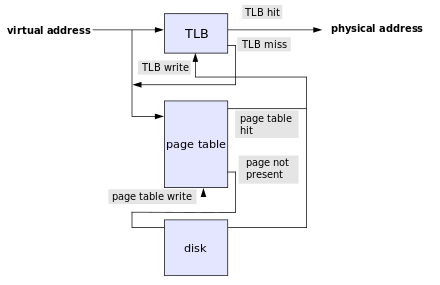
\includegraphics[scale=0.9]{./TLB.png}
\end{center}
\end{frame}
\begin{frame}
\frametitle{Fonctionnement}
Pour savoir dans quel contexte mémoire on se trouve, chaque processeur dispose d'un registre CR3, celui-ci contient l'adresse du PGD pour le processus courant. Il contient aussi les différents droits et modes des pages. 
\end{frame}
\section{Attaques}
\subsection{ATRA}
\begin{frame}
\frametitle{ATRA}
Cette attaque ne permet pas de récupérer l'adresse de la syscall table, mais on peut une fois celle-ci trouvée rendre notre rootkit plus furtif. En effet, cette attaque cherche à dupliquer la syscall table, et de faire utiliser la copie par le système.
\end{frame}
\begin{frame}
\frametitle{ATRA schéma}
\begin{center}
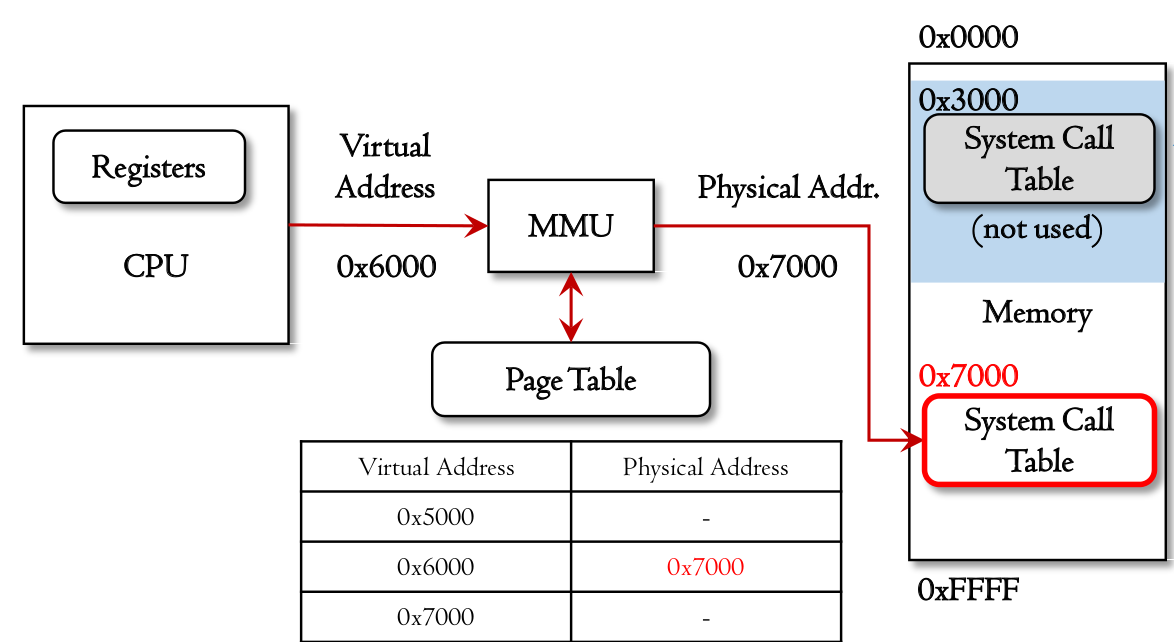
\includegraphics[scale=0.3]{./ATRA.png}
\end{center}
\end{frame}
\subsection{Attaque sur CR3}
\begin{frame}
\frametitle{CR3}
\begin{block}{}
Nous savons que les structures kernel sont partagées dans tous les processus, donc dans la mémoire de chaque processus il y a un pointeur sur la syscall table.
\end{block}
Le but de notre attaque est de retrouver la syscall en scannant les page table de notre processus et en cherchant ce pointeur.
\end{frame}

\section{Conclusion}
\begin{frame}[fragile]
\frametitle{Conclusion}
\begin{itemize}
\item 	Technique courante utilisant l'export de la fonction \textit{sys\_close}
\item 	Version 4.17 du noyau rendant cette technique obselète
\item 	Développement d'une technique alternative basée sur la recherche d'un appel à la \textit{sys\_call\_table} dans le code en mémoire
\item 	Exemple de hook de \textit{getdents} pour cacher des fichiers à l'utilisateur
\end{itemize}
\end{frame}

\section{Références}
\begin{frame}[allowframebreaks]
\frametitle{Références}
\begin{thebibliography}{}
	\bibitem{1}
	Sources du projet\\
	github.com/naka53/prime\\
	\bibitem{2}
	System calls in the Linux kernel\\
	0xax.gitbooks.io/linux-insides/content/SysCall\\
	\bibitem{3}
	Linux Kernel Sources\\
	github.com/torvalds/linux\\
	\bibitem{4}
	Memory and Page table\\
	kernel.org/doc/gorman/html/understand\\
	\bibitem{5}
	ATRA\\
	cysec.kaist.ac.kr/publications/ACM\_CCS\_2014\_ATRA.pdf\\
\end{thebibliography}
\end{frame}
\end{document}
